\chapter{Our Approach}\label{cap:our_approach}

\section{UQ Proposed Dataflow}
Summarizing, we proposed a workflow to quantify the uncertainty in large-scale spatio-temporal models, figure \ref{fig:workflow}. The workflow is divided into three main steps, the fitting process, the clustering and the queries. We illustrate the use of the workflow with  two queries, sections \ref{sub:gldMixtureWorkflow} and \ref{sub:InfomationEntropyRegionWorkflow}.

\begin{figure}[H]
    \centering
    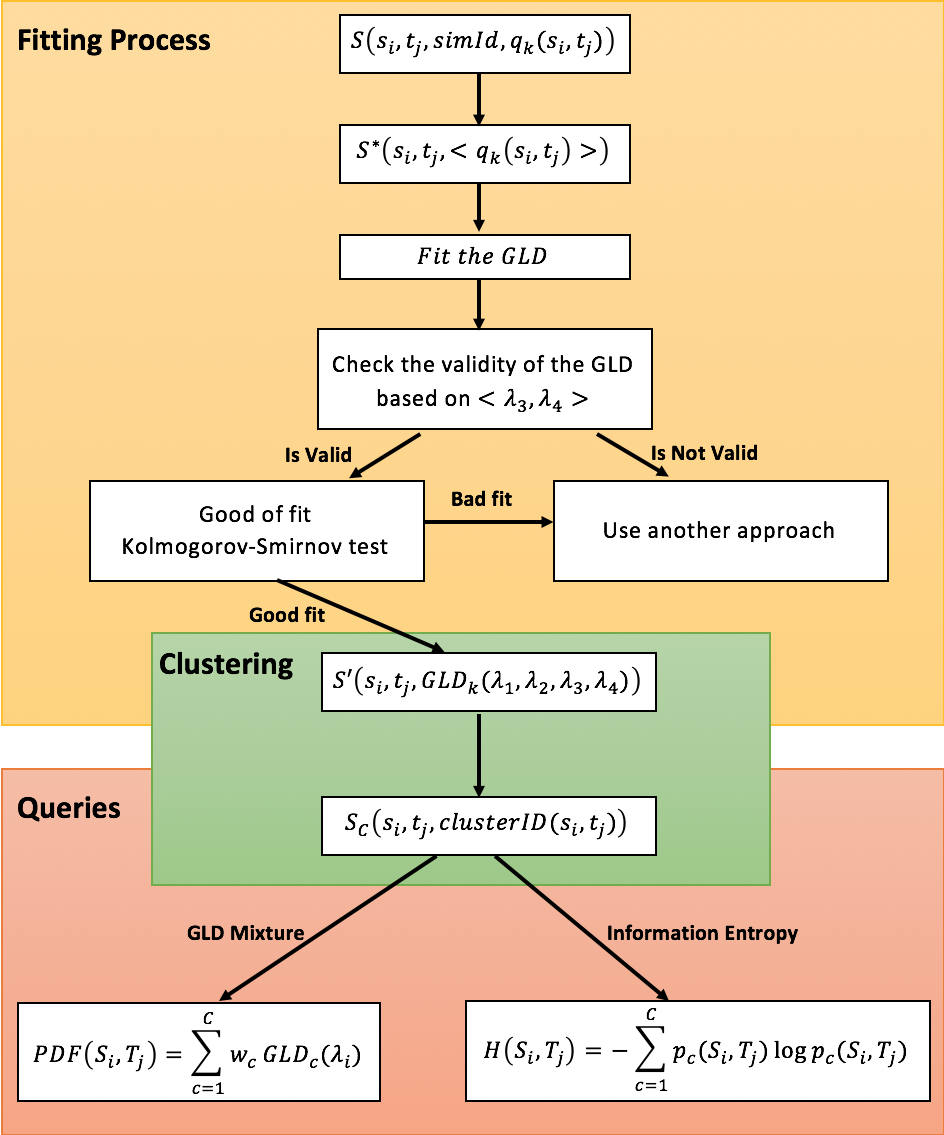
\includegraphics[width=1\textwidth]{img/Diagram.png}
    \caption{Proposed workflow. The workflow was divided in three steps, (a) the fitting process, (b) the clustering of the GLDs and, (c) the queries over the results of the clustering process.}
    \label{fig:workflow}
\end{figure}

\subsection{Clustering}
In section \ref{gldShape} we discussed the different shapes of the GLD and define the regions of the $(\lambda_{3}, \lambda_{4})$ space where the shapes are similar. In Figure \ref{fig:similarityshapesGLD}, we show how  similar values of $\lambda_{3}$ and $\lambda_{4}$ lead to similar shapes. This fact suggests that one can clusterize the \textit{GLD} based on its lambda values. The  result of this clusterization are groups of \textit{GLDs} with similar shapes (behaviors).

In addition to $\lambda_{3}$ and $\lambda_{4}$, which  represent the right and left tails of the distribution, we have also to consider $\lambda_{2}$, as the latter represents the dispersion of the distribution. 

Then, in this step of our workflow, we clusterize the \textit{GLDs} using $\lambda_{2}$, $\lambda_{3}$ and $\lambda_{4}$ values. The final result of this step is:
\begin{equation}
S_{\mathcal{C}}(s_{i},t_{j},GLD_{k},clusterID)
\end{equation}
where:
$clusterID$ represents the ID of the cluster to which the \textit{GLD} at the spatio-temporal location $(s_{i},t_{j})$ belongs.

With the \textit{GLD} clusterized, we can use this result to characterize the uncertainty in a particular spatio-temporal region, or to measure numerically the corresponding uncertainty. In subsections \ref{sub:gldMixtureWorkflow} and \ref{sub:InfomationEntropyRegionWorkflow}, we describe how those approaches are implemented (see Figure \ref{fig:workflow}).

\section{Fitting a GLD to a spatio-temporal dataset}
In the more general case the computational model $\bm{q}=\mathcal{M}(\bm{\theta})$ represents the spatio-temporal evolution of a complex systems, and the \textit{QoI} $\bm{q}$ could be represented as:  

\begin{equation} \label{eq:spatio_temporal}
\mathbf{Q} = (\mathbf{q}(s_{1},t_{1}),\mathbf{q}(s_{2},t_{2}),...,\mathbf{q}(s_{n},t_{n}))  
\end{equation}
where:
\begin{itemize}
\item $(s_{1},t_{1}),(s_{2},t_{2}),....,(s_{n},t_{n}) \in \mathcal{S} \times \mathcal{T}\subseteq\mathbb{R}^{3}\times\mathbb{R}$ represent a set of distinct spatio-temporal locations, and
\item $\mathbf{q}(s_{i},t_{j})$ represents a value of the \textit{QoI} at the spatio-temporal location $(s_{i},t_{j})$
\end{itemize}
We could have many \textit{QoI}, but for simplicity here we are going to considere just one.

In the presence of a stochastic problem, on each spatio-temporal location $(s_{i},t_{j})$ we have many realizations of $q(s_{i},t_{j})$. A structure of a database to store this information can be modeled as:
\begin{equation}\label{eq:data_base_structure}
S(s_{i},t_{j},simId,q(s_{i},t_{j}))
\end{equation}
where $simId$ represents the \textit{id} of one simulation (realization).

The first step of our approach consists of trying to find the \textit{GLD} that best fits our simulations on each spatio-temporal location. The algorithms are described in the next section.

Given a random sample $q_{1}, q_{2}, q_{3},...,q_{n}$, the basic problem in fitting a statistical distribution to these data is that of approximating the distribution from which the sample was obtained. In our approach we divide this step in three task:
\begin{itemize}
\item Fit the \textit{GLD} to the data.
\item Evaluate the validity of the resulting \textit{GLD} on each spatio-temporal location.
\item Perform a ks-test to evaluate the quality of the fit on each spatio-temporal location.
\end{itemize}

The fitting process has been implemented following the algorithm \ref{alg:fitGLD}. Before starting the fitting process, we need to group all the simulations that correspond to the same spatio-temporal location $(s_{i},t_{j})$.  As a result we get a new dataset $S^*(s_{i},t_{j},<q_1,q_2,..,q_n>)$, where $q_i, 1 \le i \le n$, represents a vector of all the values of $q$ at point $(s_{i},t_{j})$.

\subsection{Fitting process}
\label{gldFitProcess}
Now, for each spatio-temporal location $(s_{i},t_{j}) \in \mathcal{S} \times \mathcal{T}$ we use a function of the GLDEX R package described in section \ref{GLDEX}, to fit the \textit{GLD} to a vector $<q_1,q_2,..,q_n>$, line 2 of algorithm \ref{alg:fitGLD}. As a result of this task we get the lambda values of the \textit{GLD} that best fit the dataset at each spatio-temporal location, equation \ref{eq:S_GLD}.
\begin{equation}\label{eq:S_GLD}
S'(s_{i},t_{j},GLD(\lambda_{1}, \lambda_{2}, \lambda_{3}, \lambda_{4}))
\end{equation}

\subsection{GLD validity check}
As we mention in section \ref{GLD} the \textit{GLD} is not always valid, it depends of the $\lambda_{3}$  and $\lambda_{4}$ values. The evaluation of the validity of the \textit{GLD} is straightforward, if $\lambda_{3}$  and $\lambda_{4}$ are in the gray regions of Figure \ref{fig:validGLD} the \textit{GLD} is not valid, on the other case is valid.

The validity check is performed in line 3 of the algorithm \ref{alg:fitGLD}, and as a result we get:
\begin{equation}
S_{validity}(s_{i},t_{j},valid(s_{i},t_{j})),
\end{equation}
where:
\begin{equation}
  valid(s_{i},t_{j}) =
  \begin{cases}
    1 & \text{if GLD is valid in $(s_{i},t_{j})$} \\
    0 & \text{otherwise}
  \end{cases}
\end{equation}

\subsection{Quality of the fit}
\label{Quality of the fit}
Now at the remaining points, where the \textit{GLD} is valid, we need to evaluate how good is the fit. That is, we evaluate whether the \textit{GLD} (PDF) correctly describes the dataset. We use here the Kolmogorov-Smirnov test (KS-test). The KS-test  determines if two datasets differ significantly. In this case, these datasets are: the original dataset and a second one generated using the fitted GLD. As a result, this test returns two values: a Kolmogorov-Smirnoff Distance (D); and a p-value, line 5 of algorithm \ref{alg:fitGLD}. The distance D is the maximum distance between both cumulative density functions (CDF), as shown in Figure \ref{fig:D_distance}. A small distance means that both, the dataset and the fitted PDF, are similar. 

\begin{figure}[ht]
    \centering
    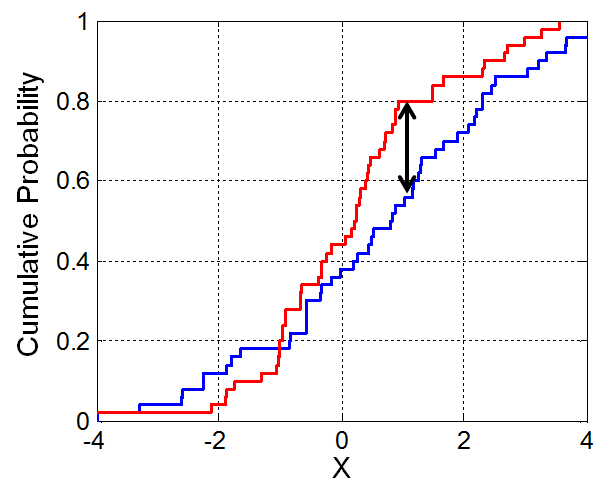
\includegraphics[width=0.45\textwidth]{img/D_distance.png}
    \caption{Illustration of the two-sample Kolmogorov–Smirnov statistic. Red and blue lines each correspond to an empirical distribution function, and the black arrow is the two-sample KS statistic.}
    \label{fig:D_distance}
\end{figure}

The second value, the p-value, is a more robust test, as it helps us to determine the significance of our results. Suppose we have two hypotheses, the null hypothesis  is that our PDF is a good fit to our dataset, and the alternative hypothesis  is that it is not. Then, a small p-value (typically $\leq 0.05)$ indicates strong evidence against the null hypothesis, so you reject the null hypothesis. A large p-value $(> 0.05)$ indicates weak evidence against the null hypothesis, so you fail to reject the null hypothesis. p-values very close to the cutoff (0.05) are considered to be marginal (could go either way). 

At the end of this task we have two new multidimensional arrays with the values of $\mathcal{D}$ and \textit{p}-value on each spatio-temporal locations.
\begin{equation}
S_{\mathcal{D}}(s_{i},t_{j},\mathcal{D}(s_{i},t_{j}))
\end{equation}
\begin{equation}
S_{p_{value}}(s_{i},t_{j},p_{value}(s_{i},t_{j}))
\end{equation}

Finally, in line 7 of the algorithm \ref{alg:fitGLD} we store the lambda values of those \textit{GLDs} that are valid and return p-values greater than 0.05.

\begin{algorithm} 
\caption{Fitting the GLD to a spatio-temporal dataset}\label{alg:fitGLD}
\begin{algorithmic}[1] 
\Function{gldFit}{$S(s_{i},t_{j},<q_1,q_2,...,q_n>)$} 
\State $<\lambda_{1},\lambda_{2},\lambda_{3},\lambda_{4}> \gets \Call {fit.gld.lm}{<q_1,q_2,...,q_n>}$

\State $isValid_{(s_{i},t_{j})} \gets \Call {validityCheck}{<\lambda_{3},\lambda_{4}>}$
\If{$isValid_{(s_{i},t_{j})}$}
\State $[pvalue,D]_{(s_{i},t_{j})} \gets \Call{ks}{<\lambda_{1},\lambda_{2},\lambda_{3},\lambda_{4}>_{(s_{i},t_{j})}}$
\EndIf
\If{$pvalue_{(s_{i},t_{j})} > 0.05$}
\State $\Call{storeLambdas}{<\lambda_{1},\lambda_{2},\lambda_{3},\lambda_{4}>,s_{i},t_{j}}$
\EndIf
\EndFunction 
\end{algorithmic} 
\end{algorithm} 

\section{Spatio-Temporal Interpolation}

\begin{tcolorbox}
\textbf{RQ2.} what is the uncertainty in some spatio-temporal locations not previously analyzed?
\end{tcolorbox}

However, adding the temporal domain implies that variability in space and time must be modelled, which is more complicated than modelling purely spatial or purely temporal variability \cite{Graler2016}.

\subsection{Kriging over GLD}

\subsection{Use Case}

\section{Queries}

\begin{tcolorbox}
\textbf{RQ4.} how to compare two regions as a function of its uncertainty?
\end{tcolorbox}

\begin{tcolorbox}
\textbf{RQ5.} what is the less uncertain model from a set of models?
\end{tcolorbox}


\subsection{Use of GLD mixture to characterize the uncertainty in an spatio-temporal region}
\label{sub:gldMixtureWorkflow}

\begin{tcolorbox}
\textbf{RQ3.} what is the uncertainty of an specific spatio-temporal region?
\end{tcolorbox}

One of the main advantages of assessing the complete probability distribution of the outputs, in place of low order moments (mean and standard deviation), is that we can use the \textit{PDFs} to answer queries. For example, suppose we want to know the mean and standard deviation in a particular spatio-temporal region $(\mathcal{S}_{i} \times \mathcal{T}_{j})$, or we want to observe graphically the distribution of the raw data generated in the simulation process in a spatio-temporal region. 

%All of this questions and many others could be answered if we have the PDFs.

%A very interesting question is, what is the face of a PDF that characterize the uncertainty in the spatio-temporal region $(\mathcal{S}_{i} \times \mathcal{T}_{j})$. 
Let us consider the second query. Up to this point, we have discussed the fit of GLDs that characterize the uncertainty at each spatio-temporal locations $(s_{i},t_{j})$, and the cluster to which the GLD at that particular spatio-temporal location would belong to. If we consider the clusterization of GLD to be of good quality, we can pick the GLD at the centroid of each cluster as a representative of all its members. In this context, in a particular spatio-temporal region, each cluster may be qualified with a weight given by:
\begin{equation}
w_{k}=\frac{1}{N}\sum_{i=1}^S \sum_{j=1}^T w(s_{i},t_{j})
\end{equation}
where:
\begin{equation}
  w(s_{i},t_{j}) =
  \begin{cases}
    1 & \text{if $clusterID(s_{i},t_{j}) = k$} \\
    0 & \text{otherwise}
  \end{cases}
\end{equation}
and  \textit{N} is the number of points in the region $(\mathcal{S}_{i} \times \mathcal{T}_{j})$.

The weight $w_k$ is the frequentist probability of occurrence of the cluster \textit{k} in the region, and complies with the conditions outlined in section \ref{GLDMixture} that $w_{k} \geq 0$ and $\sum w_{k}=1$.

Remember that the mixture of the GLDs can be written as:
\begin{equation}
f(x)=\sum_{k=1}^K w_{k}GLD(\lambda_{1},\lambda_{2},\lambda_{3},\lambda_{4})
\end{equation}
So, if we have the weights and a representative GLD for each cluster, we have the mixture of GLD that characterizes the uncertainty in the spatio-temporal region $(\mathcal{S}_{i} \times \mathcal{T}_{j})$.

The GLD mixture process is sumarized in algorithm \ref{alg:mixGLD}.

\begin{algorithm} 
\caption{GLD mixture in a region $(\mathcal{S}_{i} \times \mathcal{T}_{j})$}\label{alg:mixGLD}
\begin{algorithmic}[1] 
\Function{gldMixture}{$\mathcal{S}_{i} \times \mathcal{T}_{j}, C_{\mathcal{S}_{i} \times \mathcal{T}_{j}}$} 
%\State $K \gets \Call {clustersIn}{\mathcal{S}_{i} \times \mathcal{T}_{j}}$
\For{\textbf{each} $p_i$ in $(\mathcal{S}_{i} \times \mathcal{T}_{j})$}
\State $c \gets cluster(p_i)$
\State $w_c= w_c+1$
\State $N=N+1$
\EndFor
\State \textbf{end for}
\State \Return $\frac{1}{N} \sum_{c}^{C_{(\mathcal{S}_{i} \times \mathcal{T}_{j})}} 
    w_{c} * c.getGLD()$
\EndFunction 
\end{algorithmic} 
\end{algorithm} 

\subsection{Information entropy as a measure of the uncertainty in an spatio-temporal region}
\label{sub:InfomationEntropyRegionWorkflow}
Now, what happen if we want to measure the uncertainty quantitatively? As we mention in subsubsection \ref{subsub:informationentropytomeasuretheuncertainty} the information entropy is useful in this context. The limitation we mention in that section is solved here, because we can use the different clusters we got in section \ref{Clusterizing the GLD based in its lambda values} as the different outcomes of the system. 
The equation \ref{eq: spatio-temporal Entropy} can be rewriten as follow:
\begin{equation}\label{eq: spatio-temporal EntropyWorkflow}
H(s,t)=-\sum_{c=1}^C p_{c}(s,t)\log p_{c}(s,t)
\end{equation}
where $c$ represent a particular cluster of the total number of clusters $C$, and $p_{c}(s,t)$ represent the probability of occurence of the cluster $c$ in the spatio-temporal region $(s,t)$.

\begin{algorithm} 
\caption{Information Entropy in a region $(\mathcal{S}_{i} \times \mathcal{T}_{j})$}\label{alg:informationEntropy}
\begin{algorithmic}[1] 
\Function{gldMixture}{$\mathcal{S}_{i} \times \mathcal{T}_{j}, C_{\mathcal{S}_{i} \times \mathcal{T}_{j}}$} 
%\State $K \gets \Call {clustersIn}{\mathcal{S}_{i} \times \mathcal{T}_{j}}$
\For{\textbf{each} $p_i$ in $(\mathcal{S}_{i} \times \mathcal{T}_{j})$}
\State $c \gets cluster(p_i)$
\State $w_c= w_c+1$
\State $N=N+1$
\EndFor
\State \textbf{end for}
\State $p_{c}(s,t)= \frac{w_c}{N}$
\State $H(s, t) \gets -\sum_{c=1}^C p_{c}(s,t)\log p_{c}(s,t)$
\State \Return $H(s, t)$
\EndFunction 
\end{algorithmic} 
\end{algorithm} 

%\begin{algorithm} 
%\caption{Information Entropy in a region $(\mathcal{S}_{i} \times \mathcal{T}_{j})$}\label{alg:informationEntropy}
%\begin{algorithmic}[1] 
%\Function{infEntropy}{$\mathcal{S}_{i} \times \mathcal{T}_{j}$} 
%\For{\textbf{each} $c$ in $C$}
%\State $p_{c}(s,t) \gets \frac{1}{N}\sum_{i}^S \sum_{j}^T w(s_{i},t_{j})$
%\EndFor
%\State \textbf{end for}
%\State $H(s, t) \gets -\sum_{c=1}^C p_{c}(s,t)\log p_{c}(s,t)$
%\State \Return $H(s, t)$
%\EndFunction 
%\end{algorithmic} 
%\end{algorithm} 

Algorithm \ref{alg:informationEntropy}  computes the Information Entropy in a region $C_{(\mathcal{S}_{i} \times \mathcal{T}_{j})}$ . In lines 2 to 7, we compute the probability of each cluster in the region . Using this probability we compute the information entropy $H(s, t)$, line 8, and finally we return the result in line 9.

\subsection{Information entropy and model selection}

\section{SUQ$^2$ R package}

\section{Summary}\label{sec:approach_summary}